% Options for packages loaded elsewhere
\PassOptionsToPackage{unicode}{hyperref}
\PassOptionsToPackage{hyphens}{url}
%
\documentclass[
]{article}
\usepackage{amsmath,amssymb}
\usepackage{lmodern}
\usepackage{iftex}
\ifPDFTeX
  \usepackage[T1]{fontenc}
  \usepackage[utf8]{inputenc}
  \usepackage{textcomp} % provide euro and other symbols
\else % if luatex or xetex
  \usepackage{unicode-math}
  \defaultfontfeatures{Scale=MatchLowercase}
  \defaultfontfeatures[\rmfamily]{Ligatures=TeX,Scale=1}
\fi
% Use upquote if available, for straight quotes in verbatim environments
\IfFileExists{upquote.sty}{\usepackage{upquote}}{}
\IfFileExists{microtype.sty}{% use microtype if available
  \usepackage[]{microtype}
  \UseMicrotypeSet[protrusion]{basicmath} % disable protrusion for tt fonts
}{}
\makeatletter
\@ifundefined{KOMAClassName}{% if non-KOMA class
  \IfFileExists{parskip.sty}{%
    \usepackage{parskip}
  }{% else
    \setlength{\parindent}{0pt}
    \setlength{\parskip}{6pt plus 2pt minus 1pt}}
}{% if KOMA class
  \KOMAoptions{parskip=half}}
\makeatother
\usepackage{xcolor}
\usepackage[margin=1in]{geometry}
\usepackage{longtable,booktabs,array}
\usepackage{calc} % for calculating minipage widths
% Correct order of tables after \paragraph or \subparagraph
\usepackage{etoolbox}
\makeatletter
\patchcmd\longtable{\par}{\if@noskipsec\mbox{}\fi\par}{}{}
\makeatother
% Allow footnotes in longtable head/foot
\IfFileExists{footnotehyper.sty}{\usepackage{footnotehyper}}{\usepackage{footnote}}
\makesavenoteenv{longtable}
\usepackage{graphicx}
\makeatletter
\def\maxwidth{\ifdim\Gin@nat@width>\linewidth\linewidth\else\Gin@nat@width\fi}
\def\maxheight{\ifdim\Gin@nat@height>\textheight\textheight\else\Gin@nat@height\fi}
\makeatother
% Scale images if necessary, so that they will not overflow the page
% margins by default, and it is still possible to overwrite the defaults
% using explicit options in \includegraphics[width, height, ...]{}
\setkeys{Gin}{width=\maxwidth,height=\maxheight,keepaspectratio}
% Set default figure placement to htbp
\makeatletter
\def\fps@figure{htbp}
\makeatother
\setlength{\emergencystretch}{3em} % prevent overfull lines
\providecommand{\tightlist}{%
  \setlength{\itemsep}{0pt}\setlength{\parskip}{0pt}}
\setcounter{secnumdepth}{-\maxdimen} % remove section numbering
\ifLuaTeX
  \usepackage{selnolig}  % disable illegal ligatures
\fi
\IfFileExists{bookmark.sty}{\usepackage{bookmark}}{\usepackage{hyperref}}
\IfFileExists{xurl.sty}{\usepackage{xurl}}{} % add URL line breaks if available
\urlstyle{same} % disable monospaced font for URLs
\hypersetup{
  pdftitle={STATS 140XP Final Project EDA},
  pdfauthor={Prateik Sinha \textbar{} Jim Liu \textbar{} Ang Li \textbar{} Kris Jin \textbar{} Owen Sun \textbar{} Yixiang Gao},
  hidelinks,
  pdfcreator={LaTeX via pandoc}}

\title{STATS 140XP Final Project EDA}
\author{Prateik Sinha \textbar{} Jim Liu \textbar{} Ang Li \textbar{}
Kris Jin \textbar{} Owen Sun \textbar{} Yixiang Gao}
\date{2023-03-04}

\begin{document}
\maketitle

\hypertarget{load-in-data}{%
\section{Load in Data:}\label{load-in-data}}

\hypertarget{cleaning-data}{%
\subsection{Cleaning Data}\label{cleaning-data}}

Examining the relation between the summary and text columns:

\begin{verbatim}
## Summary:
##  My wife was driving southeast on a fairly populated main side road, it was dark out side at about 6:43pm, And my wife exclaimed” fallin 
## 
##  Text:
##  My wife was driving southeast on a fairly populated main side road, it was dark out side at about 6:43pm, And my wife exclaimed” falling star baby look quick!” When I looked up I saw not a falling star but a bright ball of light , one that was closer than any shooting star I have ever seen, it had a blue glow  changing into green colors of light as it fell from the sky. It fell as if falling from an invisible opening in the sky... the night was a crystal clear night sky  so no clouds or precipitation to obstruct our view and the object was closer than any I have ever witnessed before. The way the object fell was too slow to be a meteor or falling star, also noting that there was no “light trail” following behind the object as it fell. We watched it fall for about 5 seconds before it disappeared into the dark night sky somewhere close to the earth surface.  It was the strangest light; object; ufo... I have encountered and felt a duty to report it.
\end{verbatim}

On inspecting the data, we can see that the summary is always a
substring of the text column. Since it provides no additional
information we can remove the summary column.

Plotting each sighting on a map using its longitude and latitude, we get
the following:

\begin{figure}
\centering
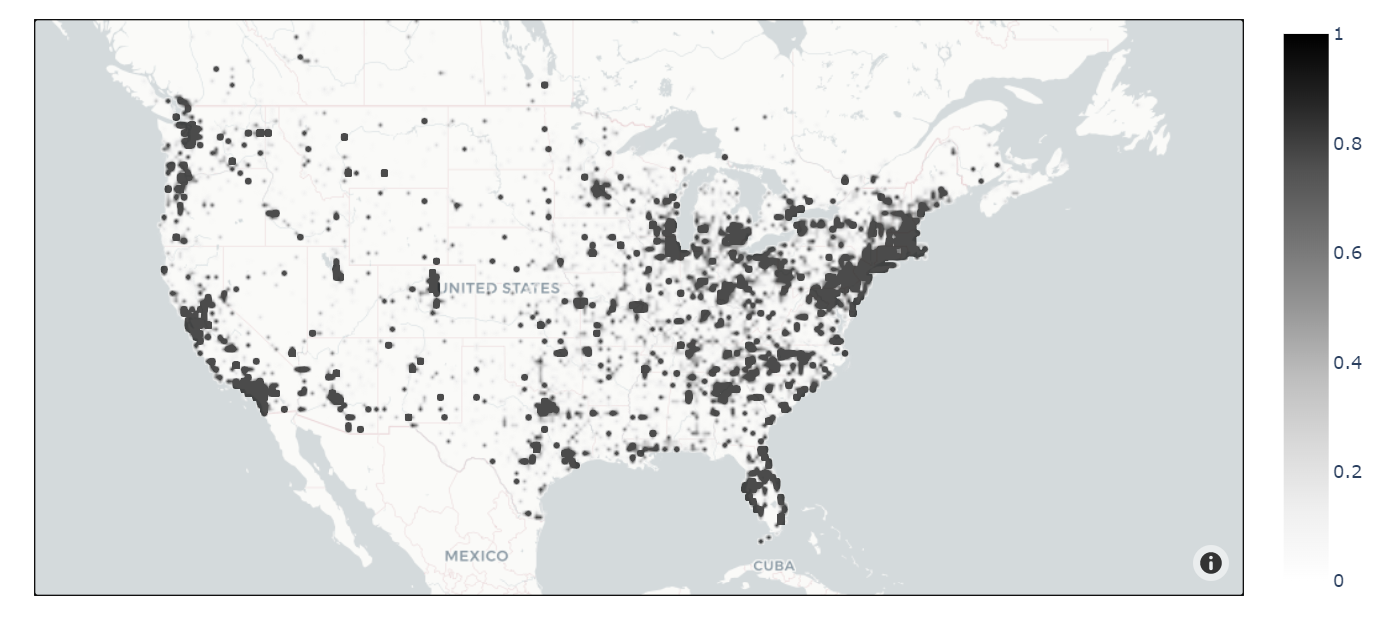
\includegraphics{ufo_map.png}
\caption{Plot of UFO sightings on map}
\end{figure}

We can see that the sightings are correlated with areas of higher
population in general, which makes sense. One thesis we could test is
checking whether these sightings happen disproportionately near areas
with US military bases, which would lend some credence to conspiracy
theories suggesting that sights such as Area 51 are areas of extra
terrestrial activity

Let us look at the distribution of these reports with respect to time:

\includegraphics{eda_files/figure-latex/unnamed-chunk-6-1.pdf}

We can see that there was a peak in the mid-2010s, with the distribution
appearing fairly normal from \textasciitilde2006 onwards. There were
very few reports before that, but these reports were submitted online
and that may be due to the fact that the internet was not as popular was
it in recent years.

Although the relative proportions of the shapes of UFOs being reported
seems to stay fairly constant throughout the years, we can look further
into which shapes are more frequent occurrences and how their popularity
changes over time:

\includegraphics{eda_files/figure-latex/unnamed-chunk-7-1.pdf}

Looking at their frequency, we can see that light is by far the most
popular, which may be due to the fact that this it is a more vague term
that could be used to describe many possible shapes rather than
something like chevron or crone, which is very specific.

The distant second place goes to circle, which may possess the same
advantage due to its abstractness. Many may describe oval, disk and egg
shapes as circles rather than place them in their own specific
categories.

The rest of the labels smoothly taper off in terms of popularity, ending
with cone and cross. Roughly 2.8346099 of the reports did not mention a
shape, meaning the vast majority of UFO encounters do have people making
clear visual contact of the vessel.

\emph{An interesting thesis to consider would be to find the relation
between the shapes and occurrences of UFOs reported by people and
coverage of them in news, media and other popular culture to see how
related they are, and if it data indicates that one may be based off
another.}

\includegraphics{eda_files/figure-latex/unnamed-chunk-8-1.pdf}

The overlapping shapes makes it harder to tell what's going on, stacking
the density plots vertically gives us:

\includegraphics{eda_files/figure-latex/unnamed-chunk-9-1.pdf}

From the above graph we can see:

\begin{itemize}
\tightlist
\item
  The vast number of different categories makes the data hard to
  analyse. Since many of these are very similar, they can be wrapped up
  into larger parent categories. For example, light, fireball and flash
  can be combined into a single category; circle, oval, egg etc. can be
  combined into another, and so on.
\end{itemize}

\begin{itemize}
\item
  The distribution appears to be tri-modal
\item
  The second mode is the largest, and contains a narrow and steep peak
  of reports, motly of light-shaped UFOs. This warrants further
  investigation into real life events at the time to see if this can be
  explained by events happening at the time.
\item
  The third peak of NA shapes seems to be the most recent. This could be
  a problem with data collection and also warrants investigation
\end{itemize}

Combining the categories, these are all the shapes that had other shapes
absorbed into them. The rest of the categories remain unchanged:

\begin{longtable}[]{@{}
  >{\raggedright\arraybackslash}p{(\columnwidth - 10\tabcolsep) * \real{0.1528}}
  >{\raggedright\arraybackslash}p{(\columnwidth - 10\tabcolsep) * \real{0.1528}}
  >{\raggedright\arraybackslash}p{(\columnwidth - 10\tabcolsep) * \real{0.1528}}
  >{\raggedright\arraybackslash}p{(\columnwidth - 10\tabcolsep) * \real{0.1667}}
  >{\raggedright\arraybackslash}p{(\columnwidth - 10\tabcolsep) * \real{0.1667}}
  >{\raggedright\arraybackslash}p{(\columnwidth - 10\tabcolsep) * \real{0.1528}}@{}}
\toprule()
\begin{minipage}[b]{\linewidth}\raggedright
Light
\end{minipage} & \begin{minipage}[b]{\linewidth}\raggedright
Circle
\end{minipage} & \begin{minipage}[b]{\linewidth}\raggedright
Triangle
\end{minipage} & \begin{minipage}[b]{\linewidth}\raggedright
Rectangle
\end{minipage} & \begin{minipage}[b]{\linewidth}\raggedright
Formation
\end{minipage} & \begin{minipage}[b]{\linewidth}\raggedright
Cylinder
\end{minipage} \\
\midrule()
\endhead
Flash

Fireball & Disk

Egg

Teardrop

Oval

Sphere & Cone & Diamond & Changing & Cigar \\
\bottomrule()
\end{longtable}

Examining the second graph again with our new shapes, and zooming to the
2nd mode:

\includegraphics{eda_files/figure-latex/unnamed-chunk-11-1.pdf}

Moving on from the shapes, next let's examine what part of the year
these sightings normally take place in to see if they are more common
during certain seasons

\includegraphics{eda_files/figure-latex/unnamed-chunk-12-1.pdf}

The sightings seem to increase slowly throughout the year, with peaks in
July, and curiously, a second peak of only chevron shaped UFOs around
November. The second peak may likely be a single event that was reported
by many people which is skewing the results and warrants further
investigation.

\hypertarget{ideas-for-research-questions}{%
\subsubsection{Ideas for research
questions:}\label{ideas-for-research-questions}}

\begin{enumerate}
\def\labelenumi{\arabic{enumi}.}
\item
  \emph{Are UFO sightings more likely to occur in certain geographic
  regions or at particular times of the year?}
\item
  \emph{Is there any correlation between reported UFO sightings and the
  presence of military installations or other government facilities?}
\item
  \emph{Can machine learning algorithms accurately classify UFO
  sightings based on their reported characteristics, such as shape or
  color?}
\item
  \emph{Are there any patterns or trends in the language used to
  describe UFO encounters, and can these patterns shed light on the
  psychological or cultural factors that contribute to belief in UFOs?}
\item
  \emph{Are there any demographic or other social factors that predict
  belief in UFOs or likelihood of reporting a sighting?}
\item
  \emph{How has media coverage and public perception of UFOs changed
  over time, and what factors have contributed to these shifts?}
\item
  \emph{Is there any evidence to suggest that UFO sightings could be
  linked to extraterrestrial life, or are there other explanations that
  can account for these phenomena?}
\end{enumerate}

\end{document}
